\chapter{Spectroscopy of EC2117-54}

\section{Observations}
\subsection{Southern African Large Telescope}
\label{SALT}

The Southern African Large Telscope (SALT) is the newest addition to the collection of telescopes operated by the South African Astronomical Observatory (SAAO). Construction has recently been completed and, although the telescope is currently in its performance verification stage, it has already produced its first scientific results \citep{salt_first_science}.

This telescope is the largest single telescope in the southern hemisphere. Its design is based on the Hobby-Eberly Telescope (HET) situated at the McDonald Observatory in Texas. The unique design of these telescopes allows for large telescopes to be built at a fraction of the cost of conventional Altitude-Azimuth (Alt-Az) telescopes. 

The telescope is unconventional in that its instruments are installed in a moving structure called the \texttt{Tracker}. The tracker moves the instruments along a theoretical surface that is concentric with the spherical surface of the main mirror. Therefore in principle it works in a similar fashion to the Arecibo radio telescope. The tracker is located at a distance of $13.08 \hspace{2pt}m$ from the primary mirror, which is half the radius of curvature. Because the primary mirror is spherical, the tracker houses a Spherical Aberration Corrector (SAC) \citep{dod2000}.

The main mirror consists of 91 hexagonal mirrors made of Astro-Sitall \citep{swiegers}. Each mirror is supported by  actuators. These are used to tip-tilt corrections of the individual mirror segments. The individual segments are also also fitted with capacitive edge sensors which are used to detect changes in the position of the individual mirrors. The changes can then be corrected. During observation, this is done at $20s$ intervals.

The primary mirror is supported by a steel structure which fixes the altitude at which the telescope points at  $37^{\circ}$. The telescope can only move in azimuth. The telescope can therefore only point to objects in an annulus in the sky at any particular moment. To observe targets outside the annulus, the operators will have to wait for these objects to move into the annulus. Objects can generally be observed twice in an evening. If the objects happen to move across the northern or southern regions of the annulus, they can be observed for longer periods ($\approx$ 4 hours) than when they move overhead from East to West ($\approx $ 1 hour on each side). To observe an object, the telescope is moved to the appropriate azimuth. The tracker is then used to follow the object as it tracks across the primary mirror.




\subsection{Robert Stobie Spectrograph}
\label{RSS}

The Robert Stobie Spectrograph (RSS), previously known as the Prime Focus Imaging Spectrograph (PFIS) is, together with SALTICAM, one of the first-generation instruments on the Southern African Large Telescope (SALT). It is a multipurpose medium resolution spectrograph. Its capabilities include medium-band imaging, Fabry-Perot imaging, longslit and multislit grating spectroscopy. High time-resolution and polarimetric modes are also possible. \citep{RSS_Modes}

A full description of the operational modes of RSS is given by \cite{RSS_Modes}. The modes relevant to this project will be summarised here.

The instrument can be seen as 4 systems in series namely the focal plane system, the dispersive elements, polarization optics and the CCD detector.

The focal plane system can be used in \textit{open}, \textit{longslit} and \textit{slitmask} mode. In \textit{open} mode there is no slitmask allowing direct imaging of objects. The \textit{longslit} mode is the standard spectroscopic mode used by most spectrographs and is also the mode used for the August 2006 observations while the \textit{slitmask} mode uses a custom laser-cut slit for multi-object spectroscopy and spectropolarimetry. \citep{RSS_Modes}

The second subsystem, the dispersive elements, comprises of an \textit{imaging mode}, \textit{Fabry-Perot} imaging mode, and a \textit{grating spectroscopy} mode \citep{RSS_Modes}. The grating spectroscopy mode was used for the August 2006 observations.

The polarization optics subsystem allows various polarimetric observations to be made. This system was not used and will not be discussed further. See \cite{RSS_Modes} and the references therein for a complete overview of this system.

The detector of the RSS comprises of 3 Marconi Applied Technologies 44-82 CCDs, each with 2048x4096 pixels of size 15 microns. The CCDs are mosaiced to form a larger detector. Each CCD has 2 amplifiers to decrease readout times. The plate scale at the detector is 117 microns/arcsec and will therefore mostly be used with 2x2 binning in order to reduce readout noise. The CCDs can be operated in 3 different modes. These are \textit{normal}, \textit{fast} and \textit{charge shuffle} modes. The \textit{normal} mode allows the entire mosaic to be read in 3.6s using 2x2 binning with 5e/pix noise \citep{RSS_Modes}. Using the frame transfer capability of the \textit{fast} readout mode, images can be obtained 1.8s apart. This is the mode used in the August 2006 observations. 


During the August 2006 observations, the telescope was still in its performance verification phase and the design specifications of RSS have not yet been met. As a result, the operation modes listed by \cite{RSS_Modes} and \cite{RSS_Opt_Design} could not be used and less than optimal observations were obtained.






\subsection{Spectroscopic observations in 2006}
\label{obs_spec}


Spectroscopic observations of EC2117-54 were made on the night of 17 August 2006 (JD 2453965) using the Robert Stobie Spectrograph (Section \ref{RSS}) by Encarni Romero-Colmenero, the on-duty SALT astronomer. A total of 335 exposures were obtained of the object as it went through eclipse. An integration time of 5s were used in order to fully sample possible lpDNOs and possibly DNOs that may occur during this time. A further $\sim5$s were needed to read out the CCDs which results in $\sim10.5$s between exposure start times. A pre-binning of 2x2 was used together with the ``bright'' gain setting, grating 0900 and a grating angle of $14.38^{\circ}$. The gain for each CCD was manually modified to avoid discontinuities in the spectra between CCDs. This is explained in Section \ref{calibrate}. A slit-width of $1.5''$ was used to minimise slit-losses. Spectra of an CuAr calibration lamp were obtained before and after the run to allow wavelength calibration and to correct for any time-dependent shifts in the instrument. The spectra obtained have a resolution of $\sim$ 0.94\AA{} over the wavelength range 3933.8\AA{} - 7022.1 \AA{}.

A spectrophotometric standard star was observed using the same instrument setup for flux calibration purposes. Absolute flux-calibration is however not possible with SALT due to the varying aperture size. These observations will only allow the shape of the spectrum to be corrected. The flux was calibrated using the middle CCD, covering the wavelength range of a Johnson V-band filter, and the simultaneous photometric observations. 

\begin{figure}
 \centering
 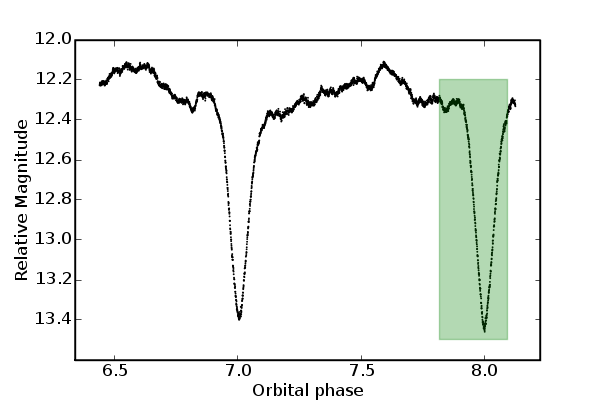
\includegraphics[width=0.9\columnwidth,bb=0 0 600 400]{images/S7655_SALT_coverage.png}
 % S7655_SALT_coverage.png: 600x400 pixel, 72dpi, 21.17x14.11 cm, bb=0 0 600 400
 \caption[Simultaneous photometry and spectroscopy]{The lightcurve of the photometric run S7655 and the simultaneous coverage of SALT high-speed spectroscopy (shaded area).}
 \label{spec_SALT_coverage}
\end{figure}




\section{Reductions}
% \subsection{Reduction of Spectroscopic Observations}
% \label{spec_reduce}

The Robert Stobie Spectrograph (RSS) is the first-generation spectrograph fitted to the SALT. It was previously known as the Prime Focus Imaging Spectrograph (PFIS). It is a medium resolution spectrograph with 3 CCD detectors. Each CCD has 2 amplifiers in order to reduce the readout time. A raw SALT RSS FITS file therefore consists of six data blocks and a single header block. In order to extract a spectrum from an image, it is necessary to perform a number of initial operations on the raw FITS file to get the data in a usable form. 

It was decided to perform the spectroscopic reductions separately on each CCD. Knowledge of the relative positions and rotations between the CCDs would therefore not be needed. Each CCD image was separately mosaiced, calibrated, extracted and wavelength calibrated. The three resulting spectra were then joined to form a single spectrum. These steps are outlined below.

The preparation of the images were performed using a script written by the author in the \texttt{Python} language. An example of it can be seen in Section \ref{pysalt}. 

\subsection{Mosaicing and Calibration}
\label{calibrate}

Each CCD has 2 amplifiers which will generally have different nominal gain settings at the time the image is read from the CCD device. The different amplifiers will therefore need to be gain-corrected separately, each with its own gain value. It was found that using the gain values specified in the FITS header resulted in an extracted spectrum that exhibited discontinuities across the boundary between different amplifiers, as well as between adjacent CCDs. This problem was fixed by calculating the median value of pixels on either side of each boundary and calculating a multiplication factor that would allow the extracted spectrum to be continuous across these boundaries. The gain factors did not need to be absolute since the extracted spectra were later flux calibrated using observations of a spectrophotometric standard star.

Each CCD was then bias-corrected using the overscan region. The median value of the overscan region was calculated and subtracted from the CCD image.

The mosaicing of these CCD images was trivial since they do not overlap. The size of the resulting image was known \textit{a priori}. A new empty image was created with dimensions $(R,2C+1)$ where $R$ is number of rows and $C$ is number of columns of each amplifier region. The two amplifier images were then added to the empty image in their correct place. The extra column inserted is the boundary between adjacent amplifiers. This empty column was filled by replacing every empty pixel by the average value of its two adjacent pixels. The bad column on CCD no. 1 was also corrected in this fashion.

Since the flatfield images had a number of saturated pixels, the spectroscopic images could not be corrected for pixel to pixel variations.

The resulting calibrated and mosaiced images were then written to disk in a new FITS file. Selected header entries copied from the primary header unit were added to each output file.

These steps were performed automatically on all raw files using the script shown in Section \ref{pysalt}.


\subsection{Spectrum Extraction}
\label{specextract}

The next step in the reduction process was to obtain wavelength- and flux-calibrated spectra from the prepared images. The extraction was done using the \texttt{IRAF} package. It was found that automating complex reductions of this nature is made difficult when using the scripting facilities in standard \texttt{IRAF}\footnote{IRAF is distributed by the National Optical Astronomy Observatory, which is operated by the Association of Universities for Research in Astronomy, Inc., under cooperative agreement with the NSF.}. Instead, \texttt{Pyraf} scripts were used to automate the spectrum extraction process. The steps followed were obtained from \cite{slitspecIRAF}.

In order to automate the reduction process, an example reduction was made manually to model subsequent reductions on. Since it was decided to separately extract and wavelength calibrate each CCD, 3 manual extractions were made for the EC2117-54 images. There was only a single exposure obtained for EG21, the spectrophotometric standard star. The extraction process for these images was completed manually using the \texttt{apall} task in \texttt{IRAF}.

The steps needed to extract an exposure are as follows:

\begin{itemize}
 \item Locate spectrum on image
 \item Trace spectrum
 \item Specifying spectrum and background windows
 \item Extraction using optimal method
 \item Extracting calibration arcs
 \item Identifying calibration arc lines and wavelength calibration
\end{itemize}

These steps were completed manually for the first exposures on each CCD. The object and background windows were specified in the interactive window of the \texttt{apall} task.

The second step, tracing the spectrum, is the process of finding the center of the object spectrum along the dispersion direction. This is necessary because any misalignment in the spectrograph, as well as the differential atmospheric refraction for different wavelengths, can cause the spectrum to not be perfectly aligned with the pixel rows on the CCD. The image columns are summed along the dispersion direction in multiple steps. For each summed column, the row number of the peak is found. The peak positions as a function of column number is then fitted with a polynomial. This function  then defines the center of the spectrum in subsequent reductions.

At this point the spectrum can be extracted from the image. The \texttt{apall} task was used for this purpose. It allows different extraction algorithms to be used. The ``Optimal'' algorithm was used to extract all the spectra. This algorithm weights every pixel according to its noise characteristics. It takes into account Poisson and readout noise. Therefore, pixels with a high signal-to-noise (S/N) ratio will be given more weight. This reduces the amount of noise in the extracted spectrum that is caused by pixels with low S/N. The details of this algorithm are given in \cite{HorneOpt}.

The calibration arcs were extracted using the same extraction window as for the object spectra. Calibration arcs of a CuAr lamp were observed before and after the run. These were used to correct for any linear shift in the instrument that may have ocurred during the observations. In order to obtain a wavelength scale for every pixel, a spline is fit to a wavelength versus pixel number plot where the wavelengths are obtained from fits to emission lines in the calibration spectra. I verified that the RMS error of the wavelength solution is $\sim 0.3$ for each spectrum. The wavelength calibration was done using the \texttt{identify} task in \texttt{IRAF}.

Subsequent exposures were extracted by using the first spectrum as starting point and then refitting the trace. The reductions were done by using the \texttt{Python} script in Appendix \ref{spec_extr}.


\subsection{Spectrum Calibration}
\label{spec_cal}

The extracted spectra now needs to be wavelength and flux-calibrated. The wavelength calibration process was done using the \texttt{identify} task in \texttt{IRAF}. This was done for a single arc spectrum. The subsequent arc spectra were wavelength-calibrated using the \texttt{reidentify} task. These tasks calculated the dispersion solution for each exposure, which were then applied to the object spectra using the \texttt{dispcor} task.

The flux calibration was based upon the spectrum of the spectrophotometric standard star, EG21 \citep{1984MNRAS.206..241B}. The sensitivity function was calculated using the \texttt{sensfunc} task and was applied to all off the EC2117-54 spectra using the \texttt{calibrate} task. Figure \ref{cal_uncal} displays the spectrum of EG21 before and after calibration.

Due to the changing pupil size of SALT, absolute flux calibration is not possible. It was decided to use the V-band photometry obtained using the SAAO 1.9m to correct for the effects of the changing pupil size. The photometric lightcurve was transformed from magnitude to intensity and was normalised by its mean. Its smoothed version, obtained from the flattening process, was used to calculate the correction. Firstly, the intensity values at the times of the spectroscopic exposures was interpolated. Then, for each of the spectroscpic exposures, the ratio of the photometric intensity and the sum of the middle CCD was calculated. This value transforms the spectroscopic flux to intensity. This value was then applied to the entire spectrum. The process is then repeated for every spectroscopic exposure.


\subsection{Signal-to-noise}
\label{signaltonoise}
The signal-to-noise (S/N) was calculated for every spectrum using the \texttt{splot} command in IRAF. Continuum regions with no detectable emission or absorption were chosen from which to calulate the S/N. The regions 6350\AA--6450\AA, 5474\AA--5574\AA\hspace{2pt} and 4450\AA--4550\AA\hspace{2pt} were chosen for the red, yellow and blue regions of the spectrum respectively. Figure \ref{snr} shows the calculated S/N as a function of orbital phase. The S/N for the blue end is significantly lower than for the red end, even though a much higher flux is expected from the blue end. At the end of the observing run, the S/N is lower than at the start. This is due to the reduction of SALT pupil size during the observations which caused an increasingly smaller amount of light to be observed thereby reducing the S/N.

In order to judge the quality of the observations, the expected S/N was calculated using the observation planning tool that is available from the SALT website\footnote{http://www.salt.ac.za/proposing/observation-planning-tools/}. The S/N was calculated for the telescope configuration at the time of the observations for a point source with magnitude V=14.7 and V=13.7 which correspond to EC2117-54 in and out of eclipse respectively. The expected S/N was calculated to be 31 for V=14.7 and 59 for V=13.7. The measured S/N of the observations is significantly lower than expected. This signal degradation was mainly caused by a seal that started leaking fluid, which in turn caused a chemical reaction in a lens, reducing its transparency severely. Measurements of the throughput suggests that the spectrograph have nominal throughput at 8000\AA, $\sim35$\% deficiency at 5500\AA \hspace{2pt} and $\sim50$\% deficiency at 4300\AA \hspace{2pt} (O'Donoghue, 2006, private communication). 

\begin{figure}
\centering
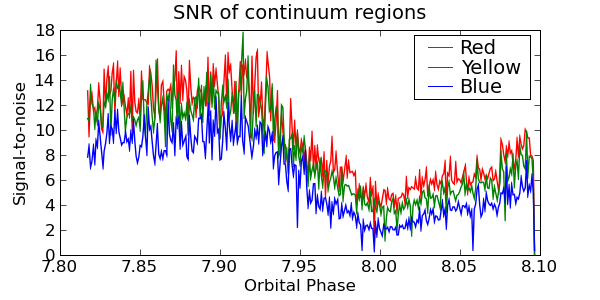
\includegraphics[width=0.8\columnwidth, bb=0 0 600 300]{spectroscopy/snr/continuum_snr.png}
\caption[Signal-to-noise curves]{Signal-to-noise (S/N) ratio as a function of orbital phase. The regions used for calculating the S/N are, Red (6350\AA--6450\AA), Yellow (5474\AA--5574\AA), Blue (4450\AA--4550\AA). } 
\label{snr}
\end{figure}


%##################################################################################################################################33

\begin{figure}
\begin{narrow}{-1in}{0in}
\begin{tabular}{cc}
 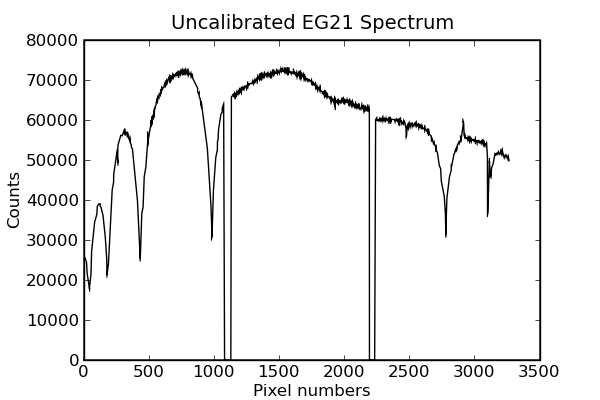
\includegraphics[width=0.65\columnwidth, bb=0 0 600 400]{images/uncalEG21.png} &
 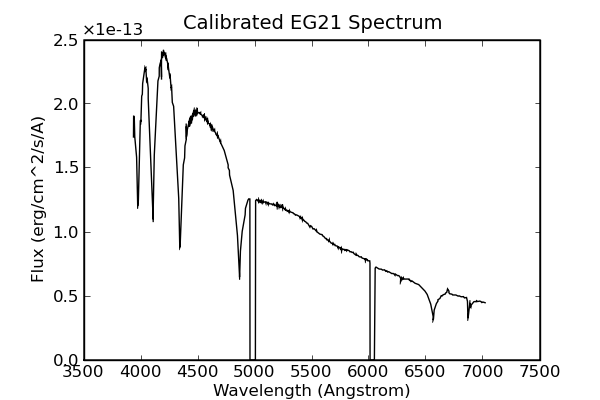
\includegraphics[width=0.65\columnwidth, bb=0 0 600 400]{images/calEG21.png} \\
\end{tabular}
\end{narrow}
\caption[EG21 spectrum before and after flux-calibration]{EG21 spectrum before and after flux- and wavelength-calibration} 
\label{cal_uncal}

\end{figure}

%##################################################################################################################################33

% \pagebreak


\pagebreak
\section{Analysis}
\label{spec_analysis}


\begin{figure}
\centering
\begin{narrow}{-1in}{0in}
 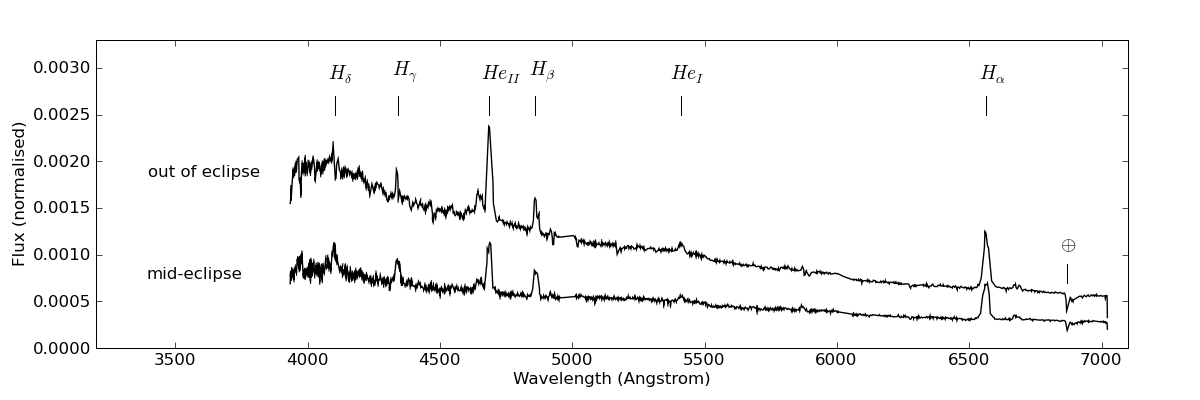
\includegraphics[width=1.4\columnwidth,bb=0 0 1200 400]{spectroscopy/spec_properties/in_out_eclipse.png}
 % in_out_eclipse.png: 1200x400 pixel, 100dpi, 30.48x10.16 cm, bb=0 0 1200 400
 
\end{narrow}
\caption[Average out-of-eclipse and mid-eclipse spectra of EC2117-54]{Average out-of-eclipse and mid-eclipse spectra of EC2117-54. The average spectrum of EC2117-54 shows broad Balmer, He I and He II lines. The out-of-eclipse spectrum (top) was obtained by averaging all spectra between orbital phases 7.817 and 7.9. During mid-eclipse (orbital phase $7.95 < \phi < 8.05$) the continuum is flatter and the He II line is comparatively weaker. The position of prominent lines and a terrestrial feature have been marked.}
\label{average_spec}
\end{figure}

%##################################################################################################################################33

\begin{figure}
\begin{narrow}{-1.2in}{0in}
 \centering
 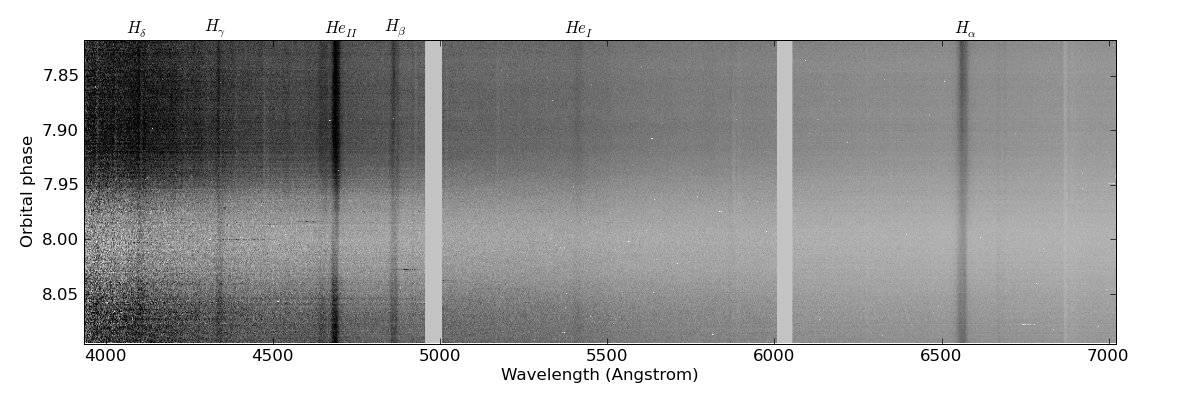
\includegraphics[width=1.5\columnwidth,bb=0 0 1200 400]{spectroscopy/final/specgram_full.png}
 % specgramHa.png: 1179666x1179666 pixel, 0dpi, infxinf cm, bb=
\end{narrow}
 \caption[Trailed spectrum for the entire spectroscopic run.]{Trailed spectrum for the entire spectroscopic run. Grayscale denotes flux level (Darker$=$higher). Important emission lines have been labelled.  }
 \label{specgram_full}
\end{figure}

%##################################################################################################################################33




\subsection{Spectral Properties}
\label{spectral_prop}

Figure \ref{average_spec} shows the average spectra of EC2117-54 in eclipse and out of eclipse. The out-of-eclipse spectrum shows broad double-peaked Balmer ($H_{\alpha}$ and $H_{\beta}$) emission and a strong He II line at 4686\AA{}. The spectra are very noisy for wavelengths bluer than $\sim5000$\AA{}. This was caused by faulty optics in the RSS that have since been repaired. This caused the higher order Balmer lines and the He II line to have a lower than expected S/N ratio. The blueshifted peaks of the Balmer lines are stronger than the redshifted peaks. This effect has been observed in other cataclysmic variables. \cite{V2051Oph2001} noted this effect in V2051 Oph but did not attempt an interpretation, other than the blue side of the accretion disk making a larger contribution to the emission. The continuum shows a steep slope towards shorter wavelengths, revealing the presence of a very hot central component in the system. The out-of-eclipse spectrum was obtained by averaging all spectra up to orbital phase 7.9.  The mid-eclipse spectrum (bottom spectrum Fig. \ref{average_spec}) was calculated by averaging the spectra between orbital phases 7.95 and 8.05. This spectrum has a flatter continuum than the out-of-eclipse spectrum.  This shows that the secondary star is cooler than the primary star and the inner regions of the accretion disk. During eclipse it contributes a greater fraction of the total light, causing a reddening of the spectrum.

% \textbf{Add some stuff about the trailed spectrograms.}









%##################################################################################################################################33

\begin{figure}
 \centering
 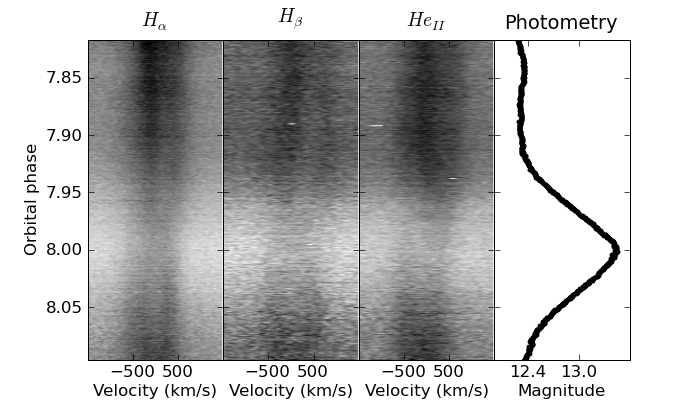
\includegraphics[width = \columnwidth, bb=0 0 700 400]{spectroscopy/final/specgram.png}
 % specgramHa.png: 1179666x1179666 pixel, 0dpi, infxinf cm, bb=
 \caption{Trailed spectrum around the $H_{\alpha}$,$H_{\beta}$ and $He_{II}$ lines.}
 \label{specgram}
\end{figure}

%##################################################################################################################################33




% %##################################################################################################################################33
% 
% \begin{figure}
% \centering
% \begin{narrow}{-1in}{0in}
% \begin{tabular}{cc}
% 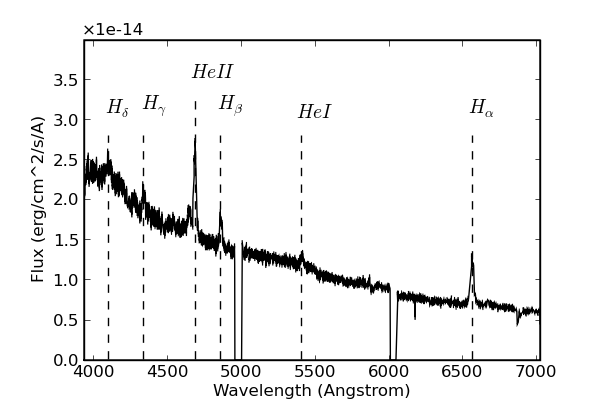
\includegraphics[width=0.65\columnwidth, bb=0 0 600 400]{images/EC2117.png} & 
% 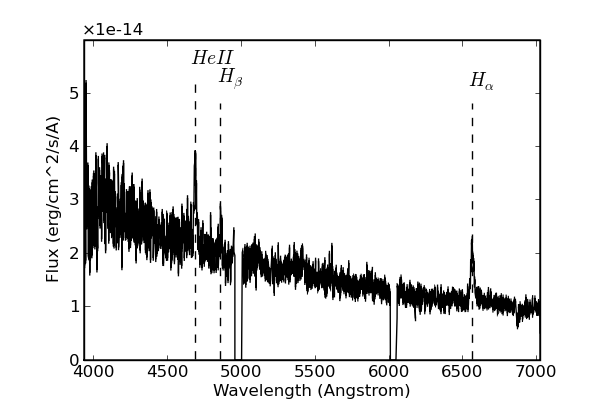
\includegraphics[width=0.65\columnwidth, bb=0 0 600 400]{images/EC0010.png} \\
% \end{tabular}
% \end{narrow}
% \caption[Single and average EC2117-54 spectra]{Left: Average EC2117-54 spectrum. Right: Single EC2117-54 spectrum. Important emission lines have been labelled.} 
% \label{EC2117ave_single}
% \end{figure}
% 
% %##################################################################################################################################33



\subsection{Time Variability}
\label{spec_timevar}

In order to study rapid time variability in the optical spectrum of EC2117-54, a number of different methods were investigated. Each spectrum was summed over all wavelengths to construct a lightcurve. The lightcurve was normalised by dividing by the mean. The periodogram of this lightcurve was inspected, but did not show any evidence for the periodicities seen in the photometric lightcurve. This suggests that the S/N ratio of the spectroscopic observations are significantly lower than the photometric observations. 
\begin{figure}[t]
 \centering
 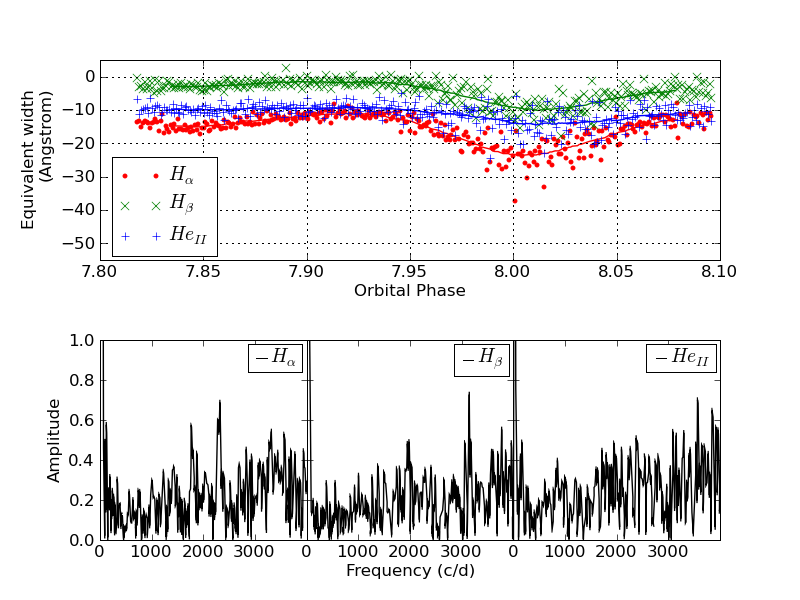
\includegraphics[width=\columnwidth,bb=0 0 800 600]{spectroscopy/lightcurves/eq_wid_lc.png}
 % eq_wid_lc.png: 800x600 pixel, 100dpi, 20.32x15.24 cm, bb=0 0 600 400
 
 \caption[Equivalent width time-series]{The equivalent width of the $H_{\alpha}$, $H_{\beta}$ and $He_{II}$ lines as a function of orbital phase (top panel) and the corresponding periodograms (bottom panels).}
\label{eq_width_lc}
\end{figure}
The equivalent width of the three most prominent lines were measured for every spectrum using the \texttt{splot} task of the \texttt{IRAF} suite. Figure \ref{eq_width_lc} shows the equivalenth width of the $H_{\alpha}$, $H_{\beta}$ and $He_{II}$ lines as a function of orbital phase and the corresponding periodograms. The Balmer lines become wider through eclipse but the He II line does not. This can be explained by examining the trailed spectrum in Fig. \ref{specgram}. The Balmer lines can be seen to have stronger emission outside eclipse. They have strong blueshifted components and  weaker redshifted components. The reason for this is unclear. During eclipse the Balmer lines become weaker but have an increased equivalent width. This was also seen in the SW Sex star, HS 0728+6738, by \cite{2004A&A...424..647R}. The equivalent width increases because the continuum source is eclipsed to a greater degree than the emission line source, suggesting that the Balmer emission originates from an optically thin region above the accretion disk. The He II line behaves differently. It stays mostly uneclipsed until $\sim$7.95 where it starts to be eclipsed. The blueshifted component is eclipsed first, as is expected from a progradely orbiting source. The fact that the ionised helium emission is nearly totally eclipsed and the eclipse duration is very short, suggests an origin in the inner regions of the accretion disk. The equivalent width curve of the He II line (Fig. \ref{eq_width_lc}) also supports this hypothesis. The equivalent width is nearly constant throughout the eclipse. The He II emission is expected to originate close to the centre of the system because the formation of higher excitation lines of helium require high temperatures. 

The possible signals detected in the periodograms in Fig. \ref{eq_width_lc} were compared to those obtained from the photometric observations. The peaks in the periodograms do not correspond to any known periodicity detected during this or previous studies of the system. The spectra were then phase-folded on all possible periods detected during this study. Because the DNOs and lpDNOs are thought to originate from rapidly rotating bright regions, a modulation that moves from the blue side of the emission lines to the red side are expected. It is assumed the bright regions rotate in a prograde direction. Folding the spectra on the oscillation period should therefore result in a diagram that shows a bright region that moves sinusoidally from the blue to red on an image that displays oscillation phase versus velocity (or equivalently, wavelength). An example of modulations in emission lines in the system V2051 Oph can be seen in Fig. 7 and Fig. 8 of \cite{V2051Oph2001}. 

Because the observations were done during the PV phase of SALT, the readout times were relatively long and low time resolution was obtained. For this reason, coupled with the throughput problems (see Section \ref{signaltonoise}), the folded spectra were averaged in 5 and 10 bins equally wide in phase space for the DNO (23.76s) and lpDNO (104.2s) signals respectively. Each bin was verified to contain approximately the same amount of spectra. No modulation at the DNO (23.76s) or lpDNO (104.2s) period is seen for any of the prominent lines. The process was repeated for all the possible periods obtained from the equivalent width curves, as well as from a lightcurve obtained by summing each full spectrum as well as each average-subtracted spectra. These are shown in the left panel of Fig. \ref{specgram_fold_ave_subDNO} and Fig. \ref{specgram_fold_ave_sublpDNO}. No evidence for modulation of the line profiles at the periods detected in the photometric lightcurves were detected. As a check, the spectra were folded on a period of 25s.  The right panel of Fig. \ref{specgram_fold_ave_subDNO} displays this plot. This plot is nearly identical to the left panel of Fig. \ref{specgram_fold_ave_subDNO} even though there are no signals detected with a period of 25s in either the photometry or the spectroscopy. This casts doubt on any systematic variations that may be seen in Fig. \ref{specgram_fold_ave_subDNO} and Fig. \ref{specgram_fold_ave_sublpDNO}. The absence of modulations in the phase-folded spectra suggests that the phase-folded spectra contain only noise and that the S/N ratio of the spectroscopic observations are indeed too low to detect the DNOs and lpDNOs or that the line modulation seen in V2051 Oph \citep{V2051Oph2001} is not present in EC2117-54.

The phase folded spectra were created from spectra at orbital phases less than 7.9. Figure \ref{snr} shows this region to have relatively high S/N (S/N $\geq$10) and therefore should show some evidence of line modulations if they are present. Contrary to this is the absence of DNOs in equivalent-width curves and lightcurves created from the spectroscopic data, suggesting that the S/N was indeed too low and that the absence of detected modulations is due to this. Although it is surprising that the spectra did not contain any evidence of rapid oscillations, it is not surprising that EC2117-54 behaves differently from V2051 Oph. V2051 Oph is classified as an SU UMa star where EC2117-54 is a nova-like. They lie on opposite sides of the period-gap and probably have very different mass-transfer rates and hence accretion disk structure. In short, there is much difference between the two systems.

\begin{figure}[ht]
\begin{narrow}{-1.25in}{0in}
\begin{tabular}{cc}
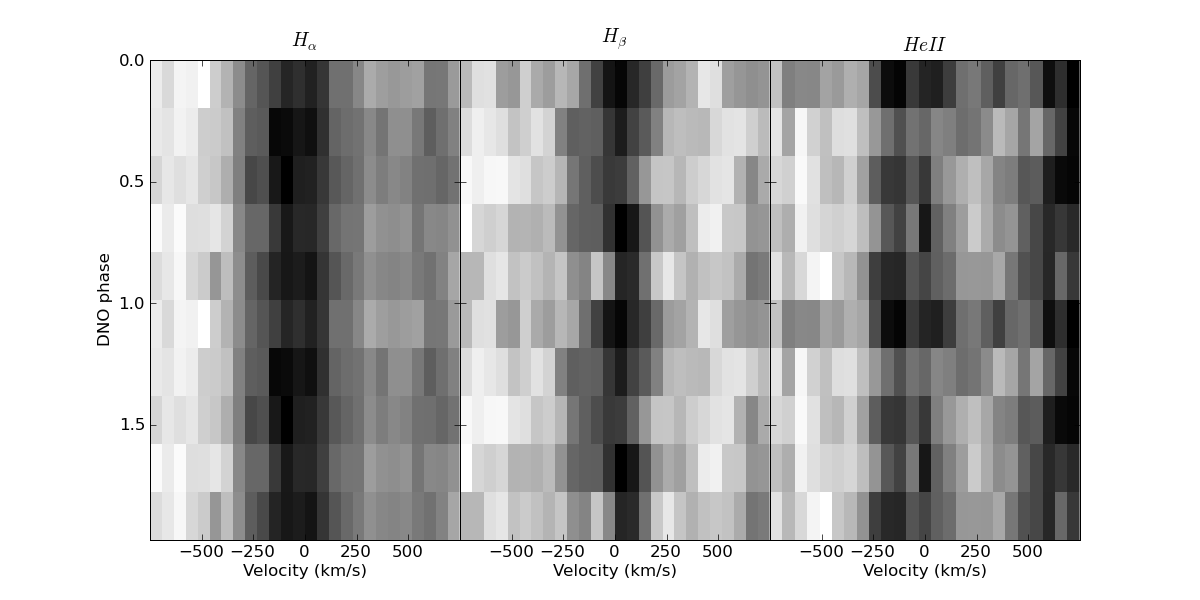
\includegraphics[width=0.7\columnwidth, bb = 0 0 1200 600]{spectroscopy/final/specgram_fold_ave_sub_DNO23.76.png} & 
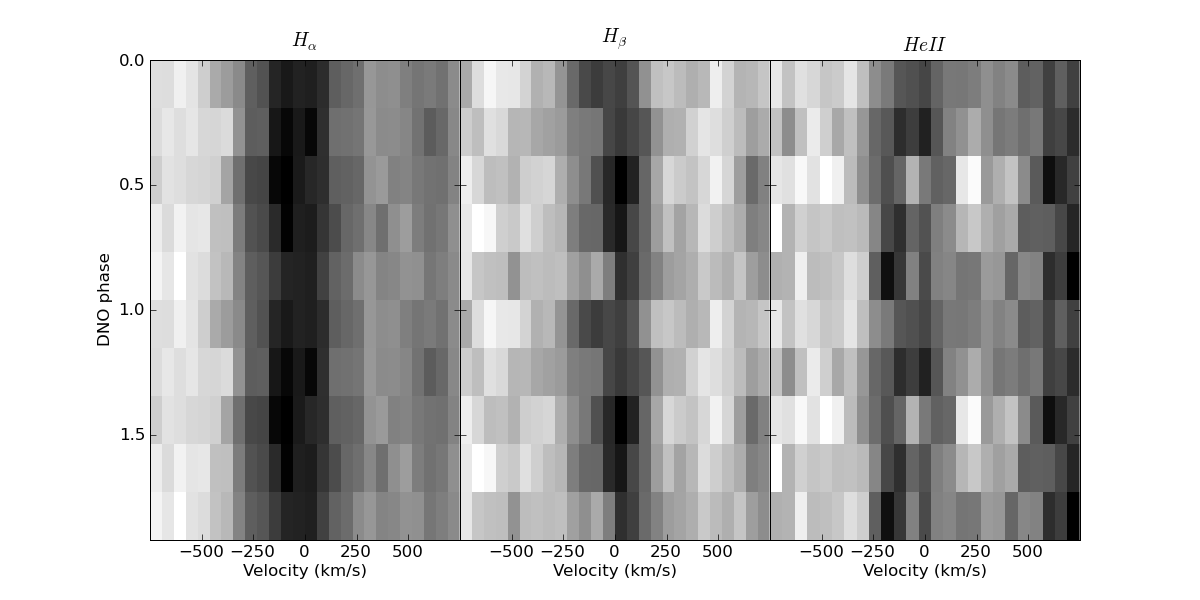
\includegraphics[width=0.7\columnwidth, bb = 0 0 1200 600]{spectroscopy/final/specgram_fold_ave_sub_DNO25.0.png}
 % specgram_fold_23.76.png: 1179666x1179666 pixel, 0dpi, infxinf cm, bb=
\end{tabular}
\end{narrow} 

\caption[Average-subtracted spectra folded on DNO period]{Average-subtracted spectra folded on DNO (23.76s) period (left panel) and mock (25.0s) period (right panel). The two plots look very similar and suggests that any no modulations can be detected at the DNO period. Black represents emission.}
\label{specgram_fold_ave_subDNO}
\end{figure}

% \begin{figure}
% \begin{narrow}{-0.in}{0in}
% \centering
%  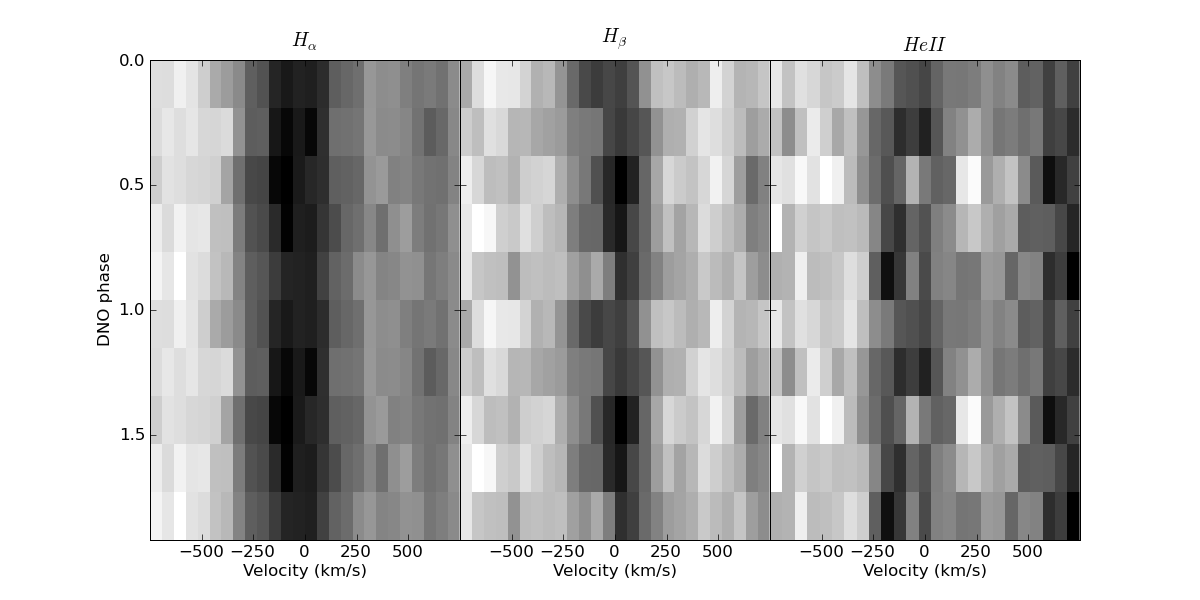
\includegraphics[width=1.0\columnwidth, bb = 0 0 1200 600]{spectroscopy/final/specgram_fold_ave_sub_DNO25.0.png}
%  % specgram_fold_23.76.png: 1179666x1179666 pixel, 0dpi, infxinf cm, bb=
% \end{narrow} 
% \caption[Average-subtracted spectra folded on DNO period]{Average-subtracted spectra folded on mock period (25.0s). Black represents emission. This plot was created to serve as a sanity-test.}
% \label{specgram_fold_ave_sub_sanity}
% \end{figure}

\begin{figure}[t]
\begin{narrow}{-0.in}{0in}
\centering
 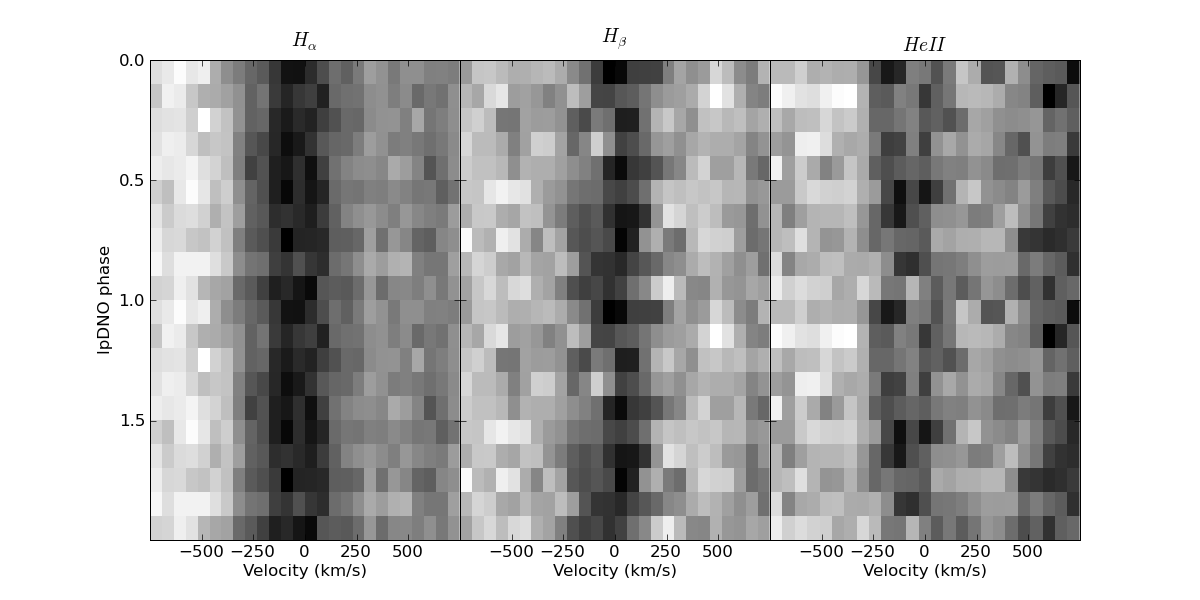
\includegraphics[width=0.7\columnwidth, bb = 0 0 1200 600]{spectroscopy/final/specgram_fold_ave_sub_lpDNO104.2.png}
 % specgram_fold_23.76.png: 1179666x1179666 pixel, 0dpi, infxinf cm, bb=
\end{narrow} 
\caption[Average-subtracted spectra folded on lpDNO period]{Average-subtracted spectra folded on lpDNO (104.2s) period. Black represents emission.}
\label{specgram_fold_ave_sublpDNO}
\end{figure}
 

% \begin{figure}
%  \centering
%  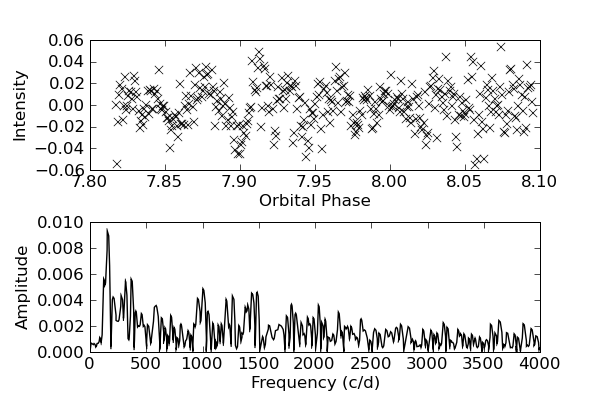
\includegraphics[width=0.8\columnwidth,bb=0 0 600 400]{spectroscopy/lightcurves/fluxlightcurve.png}
%  % fluxlightcurve.png: 600x400 pixel, 100dpi, 15.24x10.16 cm, bb=0 0 600 400
%  \caption{Lightcurve of EC2117-54 obtained from spectroscopic run}
%  \label{speclightcurve}
% \end{figure}












%##################################################################################################################################33

% \begin{figure}
% \begin{narrow}{-1in}{0in}
% \begin{tabular}{lr}
%  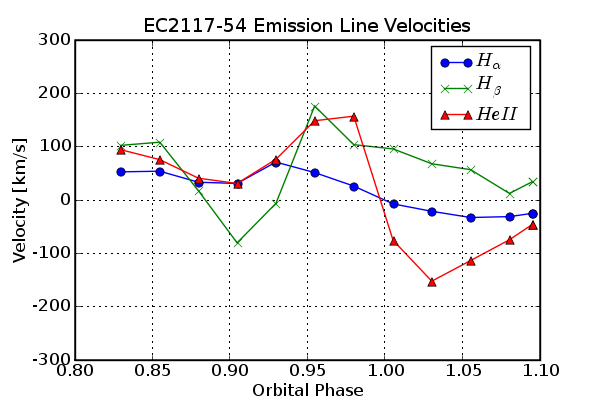
\includegraphics[width = 0.65\columnwidth, bb=0 0 600 400]{images/vel_gauss.png} &
%  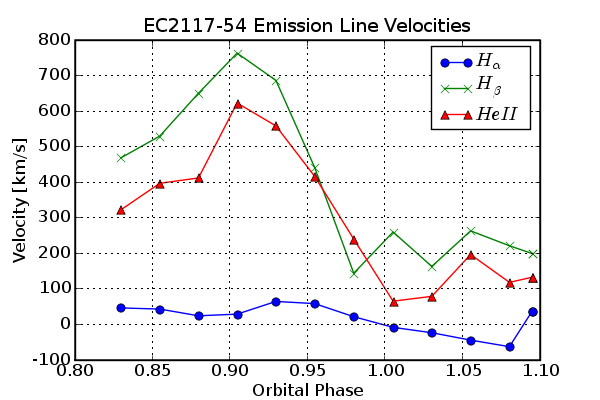
\includegraphics[width = 0.65\columnwidth, bb=0 0 600 400]{images/vel_ew.png} \\
%  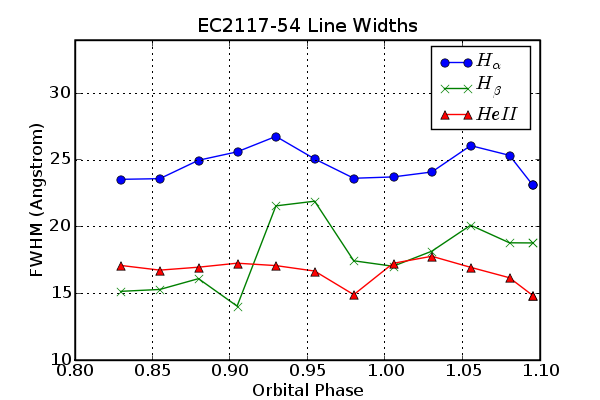
\includegraphics[width = 0.65\columnwidth, bb=0 0 600 400]{images/lw_gauss.png} &
%  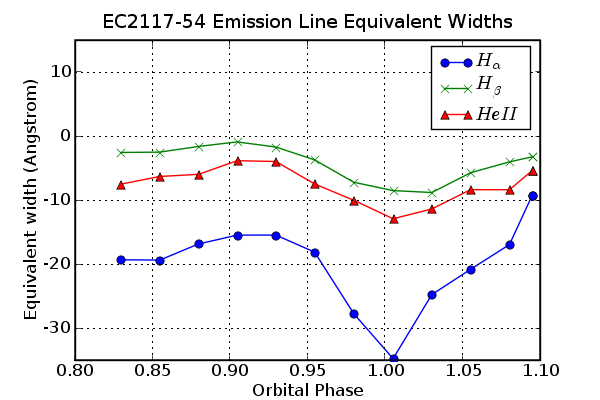
\includegraphics[width = 0.65\columnwidth, bb=0 0 600 400]{images/lw_ew.png}
% \end{tabular}
% \caption[Linewidths and velocities]{Linewidths and velocities} 
% \label{widths_velocities}
% \end{narrow}
% \end{figure}

%##################################################################################################################################33




%##################################################################################################################################33

% \begin{figure}
%  \centering
%  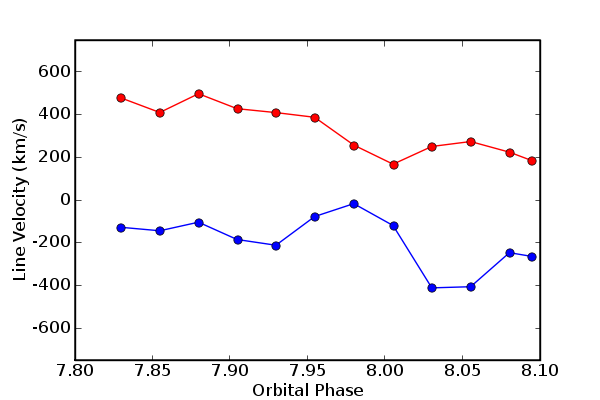
\includegraphics[width=0.9\columnwidth,bb=0 0 600 400 ]{images/ha_deblend.png}
%  % ha_deblend.png: 600x400 pixel, 72dpi, 21.17x14.11 cm, bb=0 0 600 400
%  \caption{$H_{\alpha}$ line deblended using double gaussian fit}
%  \label{ha_deblend}
% \end{figure}
% 
% \begin{figure}
%  \centering
%  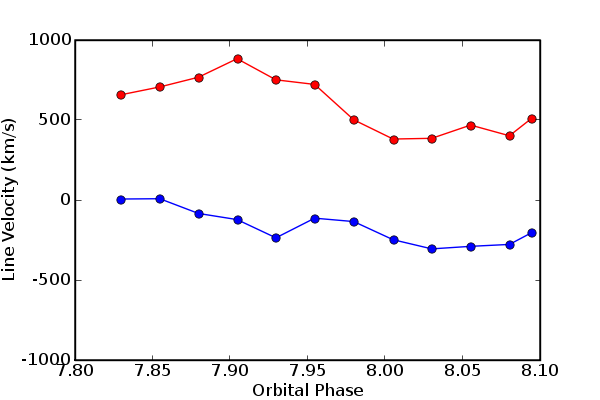
\includegraphics[width=0.9\columnwidth,bb=0 0 600 400 ]{images/hb_deblend.png}
%  % ha_deblend.png: 600x400 pixel, 72dpi, 21.17x14.11 cm, bb=0 0 600 400
%  \caption{$H_{\beta}$ line deblended using double gaussian fit}
%  \label{hb_deblend}
% \end{figure}

%##################################################################################################################################33


% \begin{figure}
% \begin{narrow}{-0.8in}{0in}
% \centering
%  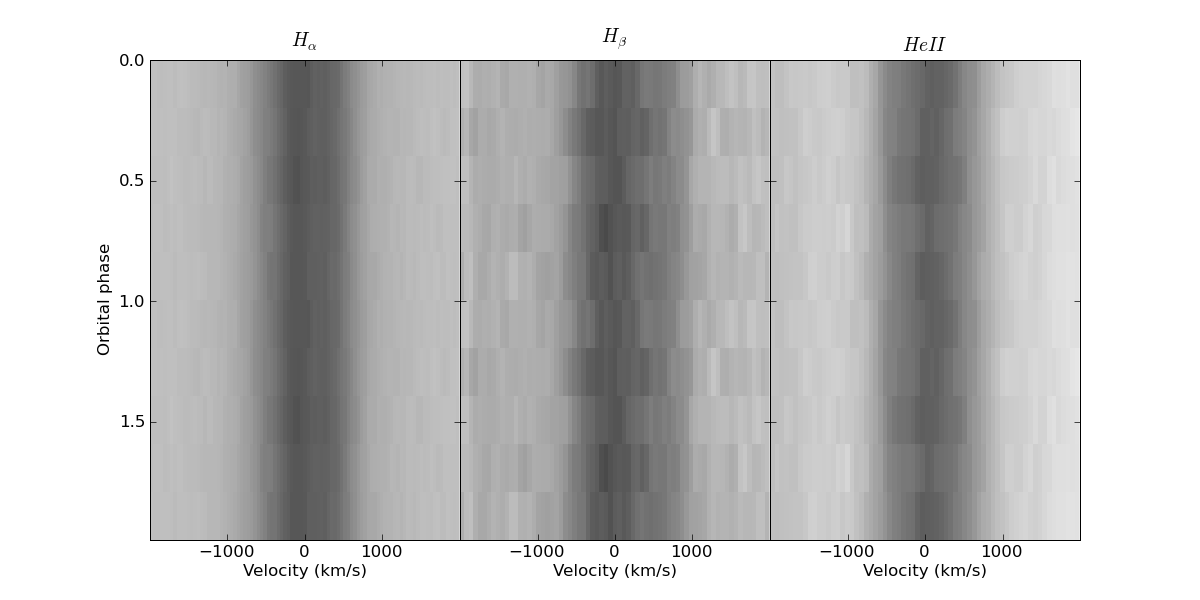
\includegraphics[width=1.2\columnwidth, bb = 0 0 1200 600]{spectroscopy/final/specgram_fold_23.76.png}
%  % specgram_fold_23.76.png: 1179666x1179666 pixel, 0dpi, infxinf cm, bb=
% \end{narrow} 
% \caption[Spectra folded on DNO period]{Spectra folded on DNO (23.76s) period. Black represents emission.}
% \label{specgram_fold_DNO}
% \end{figure}
% 
% \begin{figure}
% \begin{narrow}{-0.8in}{0in}
% \centering
%  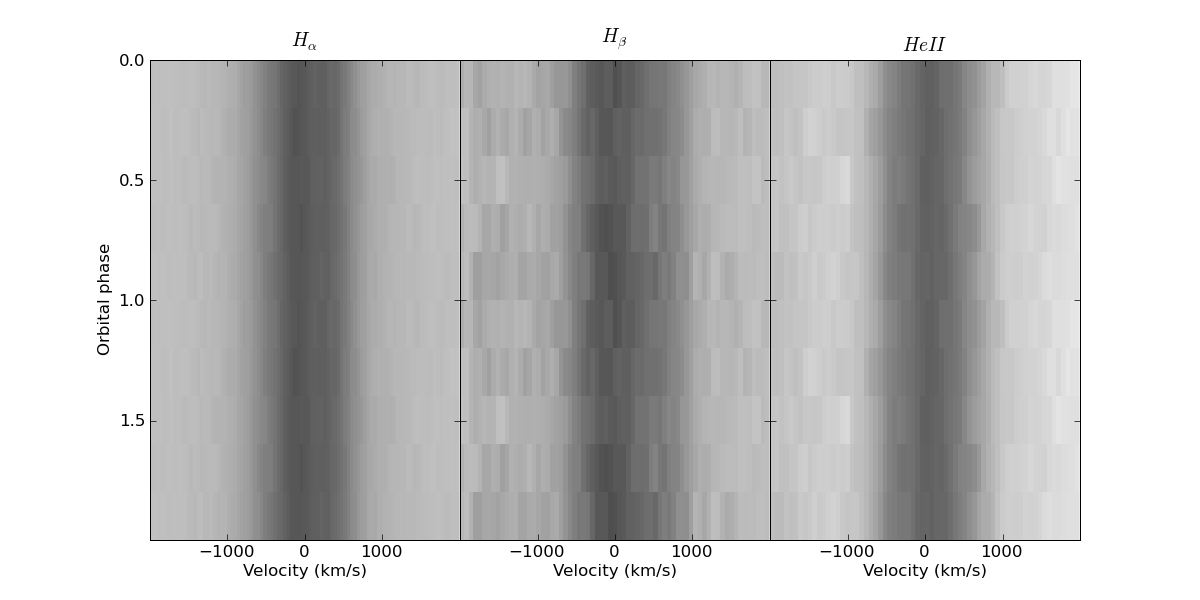
\includegraphics[width=1.2\columnwidth, bb = 0 0 1200 600]{spectroscopy/final/specgram_fold_104.2.png}
%  % specgram_fold_23.76.png: 1179666x1179666 pixel, 0dpi, infxinf cm, bb=
% \end{narrow} 
% \caption[Spectra folded on lpDNO period]{Spectra folded on lpDNO (104.2s) period. Black represents emission.}
% \label{specgram_fold_lpDNO}
% \end{figure}





